\chapter {Wizualna prezentacja projektu} 

Niniejszy rozdział poświęcony jest przedstawieniu projektu ze strony wizualnej.

Wchodząc na naszą aplikację pierwszym obrazkiem, który nas powita jest strona tytułowa wraz z zablokowanym oknem formularza, w którym będziemy mogli wpisać nazwę ubrania, do którego program będzie szukać dopasowań.

\begin{figure}[h]
    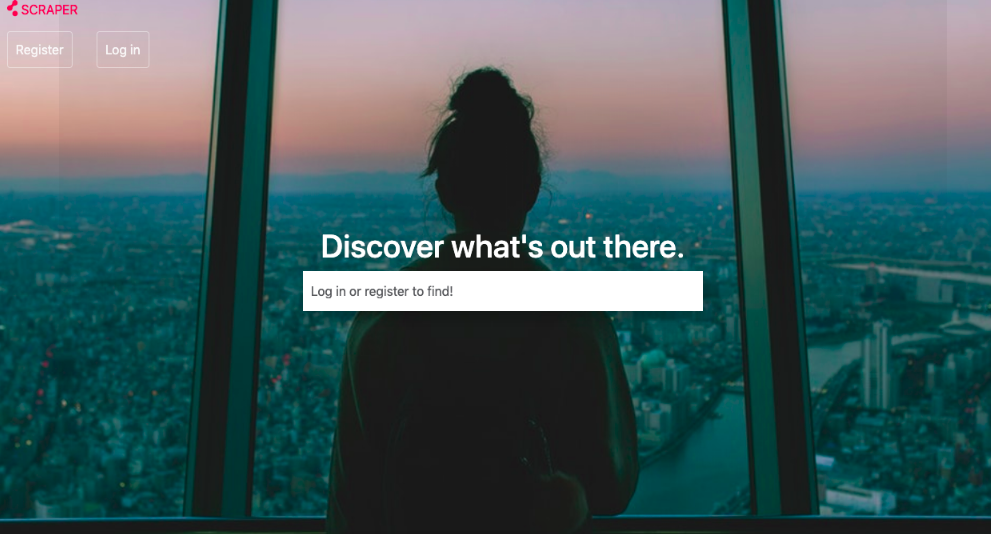
\includegraphics[width=1.10\textwidth]{zdjecia/tytulowa}
    \caption{Strona tytułowa}
\end{figure}

Użytkownik, żeby móc korzystać z aplikacji musi się zarejestrować. W tym celu klika przycisk \emph{Register}, a następnie wypełnia formularz.

\begin{figure}[h]
    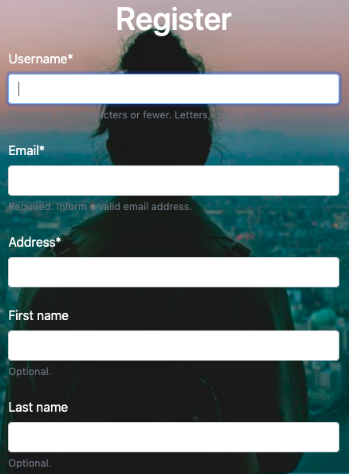
\includegraphics[height=10cm]{zdjecia/registration}
    \caption{Formularz rejestracji}
\end{figure}

\newpage
Następnym krokiem po rejestracji jest logowanie. Używając danych wpisanych podczas rejestracji można zalogować się do systemu.

Od tej chwili użytkownik może korzystać z aplikacji w stu procentach.\newline
Pojawiło się okna \emph{History} oraz \emph {Results}, w których odpowiednio można przeglądać swoją historię wyszukiwań oraz wyniki ostatniego wyszukania.
\begin{figure}[h]
    
\includegraphics{zdjecia/history_results}
    \caption{Wszystkie okna użytkownika}
\end{figure}

Jeśli przejdziemy do podstrony z historią wyszukiwań, otrzymamy widok z tabelą, która ma dwie kolumny: \emph{Name} i \emph{Date}.\newline
Tabela jest sortowalna, jest możliwość wyszukania na podstawie frazy wpisanej przez użytkownika.
\begin{figure}[h]
    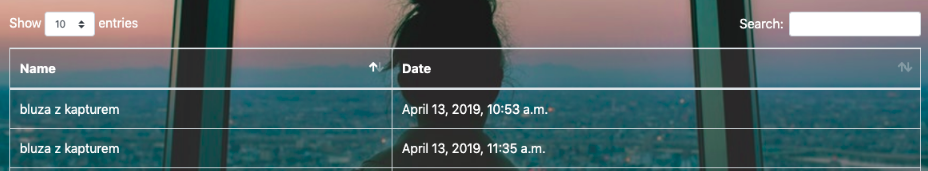
\includegraphics[width=1.10\textwidth]{zdjecia/history}
    \caption{Historia wyszukiwań}
\end{figure}
\newpage
Na stronie głównej zostało odblokowane okno z wyszukiwaniem. W tym celu można wpisać interesującą użytkownika rzecz, a następnie przejść do zakładki results, w której pojawi się tabela z nazwą ubrania, ceną, linkiem do sklepu oraz linkiem do zdjęcia. Tabela jest w pełni sortowalna, można wyszukiwać danej frazie.
\begin{figure}[h]
    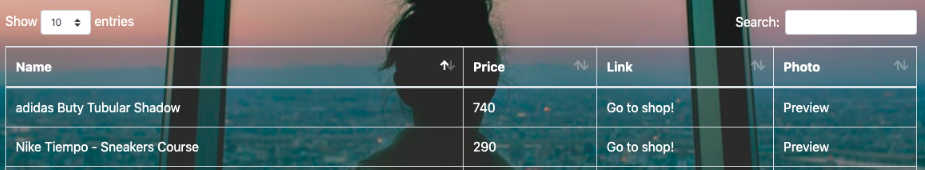
\includegraphics[width=1.10\textwidth]{zdjecia/wyniki}
    \caption{Wyniki wyszukiwań}
\end{figure}
